\documentclass{article}
\usepackage{amssymb}
\usepackage[utf8]{inputenc}
\usepackage{geometry}
\usepackage{mathtools}
\usepackage{verbatim}

\geometry{letterpaper, portrait, margin=1in}

\title{CS325 - Project 2}
\author{Group \#6 \\ William Jernigan, Alexander Merrill, Sean Rettig}
\date{\today}

\begin{document}

\maketitle

\part*{Correctness}
\section*{Proof of Claim 3: Direct Proof}

\begin{quote}
Claim 3: If $\{z_{1},z_{2},...,z_{t}\}$ and $\{z_{1}',z_{2}',...,z_{s}'\}$ are two visible sets of lines (each ordered by increasing slope), then the visible subset of $\{z_{1},z_{2},...,z_{t}\}\cup\{z_{1}',z_{2}',...,z_{s}'\}$ is $\{z_{1},...,z_{i}\}\cup\{z_{j}',...,z_{s}'\}$ for some $i \geq 1$ and $j \leq s$.
\end{quote}
Let $A = \{a_{1},a_{2},...,a_{t}\}$ be the set $\{z_{1},z_{2},...,z_{t}\}$ and let $B = \{b_{1},b_{2},...,b_{s}\}$ be the set $\{z_{1}',z_{2}',...,z_{s}'\}$ for improved clarity.

\subsection*{Prove that $\{a_{1},...,a_{i}\}$ is visible:}
    Because all elements in A were defined to be visible with respect to each other, any covering line $b_{q}$ must be from B.\\
    Given that $m_{a_{t}} < m_{b_{1}}$, a covered line $a_{p} \in A$ has $m_{p} < m_{q}$.
    
    \subsubsection*{Prove that for any covered line $a_{p}$, all lines to the right of p in A are also covered:}
        Because $a_p$ is defined to be invisible, then by Claim 2 in the P1 Visible Lines Handout:\\
        $y_{a_{p-1}}(x_{a_{p-1}, b_{q}}) > y_{a_{p}}(x_{a_{p-1},b_{q}})$, where $x_{a_{p-1}, b_{q}}$ is the x coordinate where $a_{p-1}$ and $b_q$ intersect.\\
        Because $a_{p+1}$ is defined to not cover $a_p$, we know that $y_{a_{p}}(x_{a_{p-1}, b_{q}}) > y_{a_{p+1}}(x_{a_{p-1},b_{q}})$.\\
        For $x < x_{a_{p-1},a_{p}}, a_{p+1}$ is covered by $a_p$.\\
        We need to show that $a_{p+1}$ is covered for $x \geq x_{a_{p-1},a_{p}}$.\\
        Because $b_q$ is covering $a_p$, $y_{b_{q}}(x) > y_{a_{q}}(x)$ for $x \geq x_{a_{p-1},b_{q}} \geq x_{a_{p-1},a_{p}}$.\\
        $\therefore p+1$ is invisible if p is invisible.\\
        This follows for all p.\\
        Then let $p = i + 1$.\\
        $\therefore \{a_1,...,a_i\}$ is visible and $\{a_p,...,a_t\}$ is invisible.\\

\subsection*{Prove that $\{b_{j},...,b_{s}\}$ is visible}
    Because all elements in B were defined to be visible with respect to each other, any covering line $a_{o}$ must be from A.\\
    Given that $m_{a_{t}} < m_{b_{1}}$, a covered line $b_{r} \in B$ has $m_{o} < m_{r}$.
    
    \subsubsection*{Prove that for any covered line  $b_{r}, r = s - 1$, all lines to the left of r in B are also covered:}
        Because $a_p$ is defined to be invisible, then by Claim 2 in the P1 Visible Lines Handout:\\
        $y_{b_{r+1}}(x_{b_{r+1}, a_{o}}) > y_{b_{r}}(x_{b_{r+1},a_{o}})$, where $x_{b_{r+1}, a_{o}}$ is the x coordinate where $b_{r+1}$ and $a_o$ intersect.\\
        Because $b_{r-1}$ is defined to not cover $b_r$, we know that $y_{b_{r}}(x_{b_{r+1}, a_{o}}) > y_{b_{r-1}}(x_{b_{r+1},a_{o}})$.\\
        For $x < x_{b_{r+1},b_{r}}, b_{r-1}$ is covered by $b_r$.\\
        We need to show that $b_{r-1}$ is covered for $x \geq x_{b_{r+1},b_{r}}$.\\
        Because $a_q$ is covering $b_r$, $y_{a_{o}}(x) > y_{b_{o}}(x)$ for $x \geq x_{b_{r+1},a_{o}} \geq x_{b_{r+1},b_{r}}$.\\
        $\therefore r-1$ is invisible if r is invisible.\\
        This follows for all r.\\
        Then let $r = j - 1$.\\
        $\therefore$ $\{b_j,...,b_s\}$ is visible and $\{b_1,...,b_{r}\}$ is invisible.\\

\section*{Proof of MergeVisible: Direct Proof}

\subsection*{Prove that for each line that MergeVisible checks, it correctly determines the visibility of the line:}
For each line at $i$ that MergeVisible checks, it chooses $j, k$ with $j < i < k$ and marks the line as invisible if $y_j (x_{j,k}) > y_i(x_{j,k})$.\\
Therefore, by the proof of Claims 2 and 3 in the "Visible Line Notes" handout, each line it checks and marks as invisible is actually invisible.\\
Additionally, for each line that MergeVisible checks the visibility of, it also checks to make sure that the previous line was not covered by the current line (using the same check), thereby exhausting all possible combinations of $j, k$.\\
Therefore, there is no $i$ such that $j < i < k$ and $y_j (x_{j,k}) > y_i(x_{j,k})$.\\
Therefore, by the proof of Claims 2 and 3 in the "Visible Line Notes" handout, every line marked as visible is actually visible.

\subsection*{Prove that each line in the rest of each set is also invisible if an invisible line is found:}
By the proof of Claim 3, we know that if a line in $A$ with index $p$ is invisible, then all lines in $A$ with index $> p$ are also invisible.\\
By the proof of Claim 3, we know that if a line in $B$ with index $r$ is invisible, then all lines in $B$ with index $< r$ are also invisible.

\section*{Proof of Algorithm 4: Proof by Induction}
    Let $Y$ be a list of $n$ lines sorted in ascending order by slope.  We claim that Algorithm 4 will return the visible subset of $Y$.
    \subsection*{Base case:}
    For any set of size $< 2$, we know that each line in the set is trivially visible because no other lines exist to cover the single line in the set.
    \subsection*{Inductive hypothesis:}
    By our proof of MergeVisible, we know that if MergeVisible is passed two sets of visible lines, that it will correctly return the merged set of visible lines.
    \subsection*{Applying the axiom of induction:}
    Because Algorithm 4 subdivides the given set of lines $Y$ into sets of size 1 (which are visible according to the base case) before passing them to MergeVisible, we know that the result of each first MergeVisible call is correct.\\
    Because Algorithm 4 then only passes the results of correct previous MergeVisible calls to MergeVisible, each subsequent call of MergeVisible also returns a correct result.\\
    Therefore, once all subsets of $Y$ have been merged using MergeVisible, we know that the result of the final MergeVisible call is correct.\\
    Therefore, because Algorithm 4 returns this result, we know that Algorithm 4 correctly returns the set of visible lines given any set of lines $Y$.

\section*{Experimental and Asymptotic Run Time Analysis}
\subsection*{Experimental Run Time Data}
\verbatiminput{times.txt}

\pagebreak

\subsection*{Experimental Run Time Plots}
\centerline{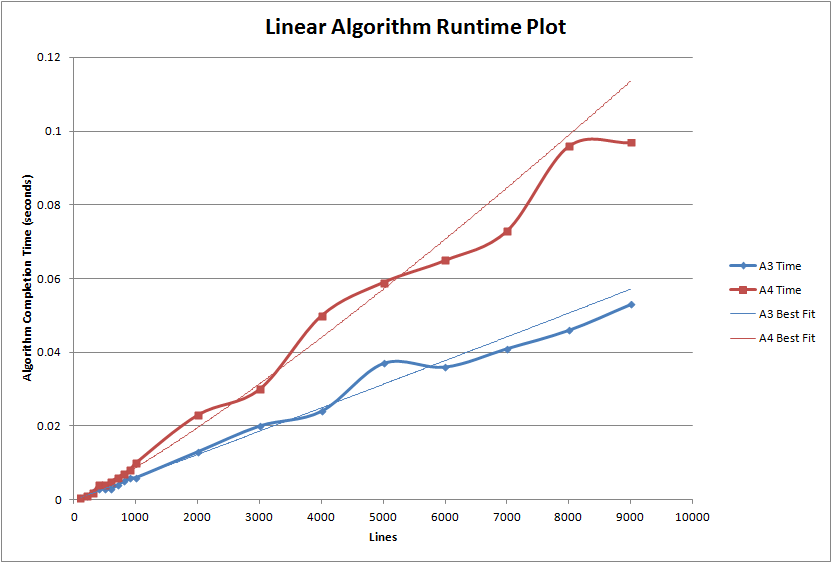
\includegraphics[width=0.75\textwidth]{plot1.png}}
\centerline{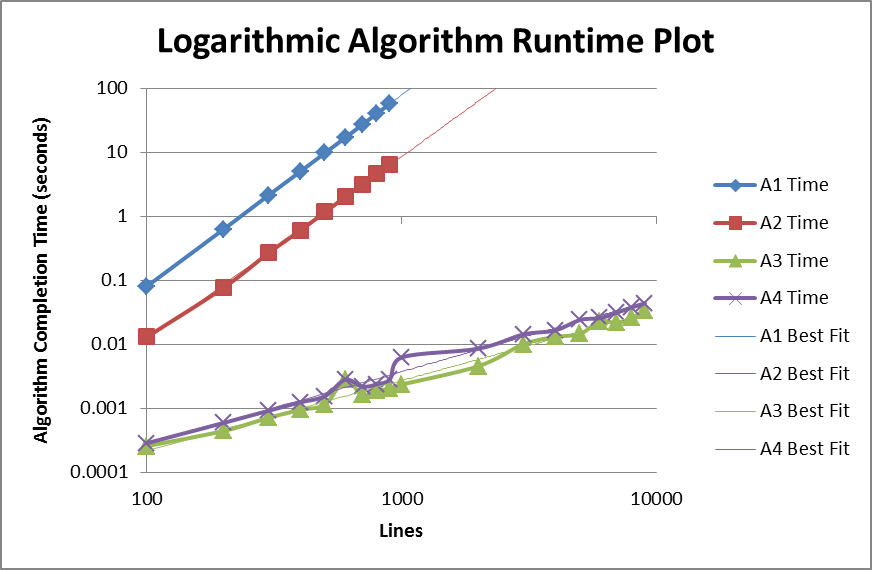
\includegraphics[width=0.75\textwidth]{plot2.png}}

\pagebreak

\subsection*{Experimental Run Time Analysis}
Algorithm 1: $y=8 \times 10^{-8}x^{3.0026}$\\
Algorithm 2: $y=4 \times 10^{-8}x^{2.7892}$\\
Algorithm 3: $y=1 \times 10^{-6}x^{1.0921}$\\
Algorithm 4: $y=2 \times 10^{-6}x^{1.1231}$\\

Given these equations, we can use both the slopes and our code to analyze the run times of the algorithms. We can also determine the biggest instance that can be solved with each algorithm in an hour.

\subsection*{Asymptotic Run Time Analysis}
Algorithm 1: $\Theta(n^3)$\\
Algorithm 2: $\Theta(n^3)$\\
Algorithm 3: $O(n^2), \Omega(n)$\\
Algorithm 4: $O(n\log n), \Omega(\log n)$\\

\subsection*{Extrapolation and Interpretation}
\subsubsection*{Estimated Number of Lines Per Hour}
Algorithm 1: $\sim 3,532$\\
Algorithm 2: $\sim 8,460$\\
Algorithm 3: $\sim 562,848,000$\\
Algorithm 4: $\sim 174,111,000$

\subsubsection*{Discrepancies}
%The theoretical run-time for Algorithm 4 is theoretically faster than that of Algorithm 3 however the experimental run-time is slower. This is likely due to how Python and the processor handle our code. Since both have linear run-times, it's likely that the constants for Algorithm 4 are largely, which could be due to how our code is handled by the Python compiler or how it's processed. For example, this could be due to Algorithm 4 creating more arrays than Algorithm 3 and creating and tearing down arrays being more time intensive.

We note that the slopes from our experimentally-derived equations are within the asymptotic run-time range of $O(n^2)$, $\Omega(n)$ and $O(n\log n)$, $\Omega(\log n)$.  However, our implementation of Algorithm 4 actually seems to run slightly slower compared to our Algorithm 3, despite Algorithm 4 having smaller minimum and maximum asymptotic runtimes.  This discrepancy has many possible contributing factors, including a small sample size, differences in how the compiler and system the operations performed in each algorithm, the randomness of the input data sets.  This randomness is due to both algorithms not performing a fixed number of operations, but rather changing what operations they run depending on the input lines given.  It is possible that our tests are biased toward data sets that provide an advantage to Algorithm 3 (or a disadvantage to Algorithm 4).  This randomness and compiler/system code handling are likely the primary causes of these differences.

\pagebreak

\section*{Pseudocode}
\verbatiminput{pseudocode.txt}

\end{document}
